%% bare_jrnl.tex
%% V1.4a
%% 2014/09/17
%% by Michael Shell
%% see http://www.michaelshell.org/
%% for current contact information.
%%
%% This is a skeleton file demonstrating the use of IEEEtran.cls
%% (requires IEEEtran.cls version 1.8a or later) with an IEEE
%% journal paper.

\documentclass[journal]{IEEEtran}

\usepackage[utf8]{inputenc}
\usepackage{hyperref}
\usepackage{graphicx}
\usepackage{booktabs}
\usepackage{multirow}
\usepackage{xcolor}
\usepackage{cite}
\usepackage{epstopdf}
\usepackage{array}

\hypersetup{hidelinks}

\renewcommand{\figureautorefname}{Figura}

\begin{document}
%
% paper title
% Titles are generally capitalized except for words such as a, an, and, as,
% at, but, by, for, in, nor, of, on, or, the, to and up, which are usually
% not capitalized unless they are the first or last word of the title.
% Linebreaks \\ can be used within to get better formatting as desired.
% Do not put math or special symbols in the title.
\title{PADE: Desenvolvimento e Validação de uma Plataforma de Sistema Multiagente para Aplicação em Redes Elétricas Inteligentes}
%
%
% author names and IEEE memberships
% note positions of commas and nonbreaking spaces ( ~ ) LaTeX will not break
% a structure at a ~ so this keeps an author's name from being broken across
% two lines.
% use \thanks{} to gain access to the first footnote area
% a separate \thanks must be used for each paragraph as LaTeX2e's \thanks
% was not built to handle multiple paragraphs
%

\author{R.~F.~Sampaio,
        L.~S.~Melo,
        R.~P.~S.~Leão,
        and ~G.~C.~Barroso% <-this % stops a space
\thanks{R. F. Sampaio, L. S. Melo and R. P. S. Leão are with the Department
of Electrical Engineering, Federal University of Ceará, Fortaleza,
CE, Brazil}% <-this % stops a space
\thanks{G. C. Barroso is with Department of Physics, Federal University of Ceará, Fortaleza, CE, Brazil}% <-this % stops a space
\thanks{Manuscript received Month day, year; revised Month day, year.}}

% note the % following the last \IEEEmembership and also \thanks - 
% these prevent an unwanted space from occurring between the last author name
% and the end of the author line. i.e., if you had this:
% 
% \author{....lastname \thanks{...} \thanks{...} }
%                     ^------------^------------^----Do not want these spaces!
%
% a space would be appended to the last name and could cause every name on that
% line to be shifted left slightly. This is one of those "LaTeX things". For
% instance, "\textbf{A} \textbf{B}" will typeset as "A B" not "AB". To get
% "AB" then you have to do: "\textbf{A}\textbf{B}"
% \thanks is no different in this regard, so shield the last } of each \thanks
% that ends a line with a % and do not let a space in before the next \thanks.
% Spaces after \IEEEmembership other than the last one are OK (and needed) as
% you are supposed to have spaces between the names. For what it is worth,
% this is a minor point as most people would not even notice if the said evil
% space somehow managed to creep in.



% The paper headers
\markboth{Transactions on Smart Grid,~Vol.~xx, No.~x, Month~2015}%
{Furtado \MakeLowercase{\textit{et al.}}: Automatic Restoration System for Power Distribution Networks Based on Multi-Agent Systems}
% The only time the second header will appear is for the odd numbered pages
% after the title page when using the twoside option.
% 
% *** Note that you probably will NOT want to include the author's ***
% *** name in the headers of peer review papers.                   ***
% You can use \ifCLASSOPTIONpeerreview for conditional compilation here if
% you desire.




% If you want to put a publisher's ID mark on the page you can do it like
% this:
%\IEEEpubid{0000--0000/00\$00.00~\copyright~2014 IEEE}
% Remember, if you use this you must call \IEEEpubidadjcol in the second
% column for its text to clear the IEEEpubid mark.



% use for special paper notices
%\IEEEspecialpapernotice{(Invited Paper)}




% make the title area
\maketitle

% As a general rule, do not put math, special symbols or citations
% in the abstract or keywords.
\begin{abstract}
Smart Grid (SG) compreende uma rede elétrica com fluxo bidirecional, integrada a uma infraestrutura composta de sistemas de comunicação, proteção, controle e monitoramento, baseados em sensores e dispositivos inteligentes, com processamento e funções distribuídas, responsáveis pela automação dos seguimentos de geração, transmissão, distribuição, abrangendo prosumidores e consumidores. A capacidade de modelagem, simulação e desenvolvimento de sistemas distribuídos, baseados em padrões que garantem a interoperabilidade entre sistemas e dispositivos, tornaram a tecnologia de Sistemas Multiagentes (MAS) uma técnica promissora para aplicação em SG. Dentro deste contexto, neste trabalho é proposta a especificação e implementação da platforma Phyton Development Agent (PADE), construída com base nas especificações da Foundation for Intelligent Physical Agents (FIPA) e concebida para desenvolvimento de funções distribuídas, com inteligência embarcada, aplicadas às SG. A FIPA é uma entidade que estabelece padrões de aplicações, arquitetura, comunicação, gerência e transporte de mensagens para desenvolvimento de plataformas e MAS, de forma a garantir a interoperabilidade entre os agentes. Além da PADE, também é proposto um Sistema Multiagente para Recomposição de Rede de Distribuição de Energia (MARS) desenvolvido para teste e validação do PADE. O MARS foi implantado em diferentes plataformas computacionais e integradas via rede local aos IED de proteção, no laboratório de redes elétricas inteligentes da Universidade Federal do Ceará. Os testes realizados com o MARS integrado aos IED de proteção padrão IEC 61.850 evidenciaram o potencial da plataforma PADE para desenvolvimento de funções inteligentes e distribuídas aplicadas às SG.
\end{abstract}

% Note that keywords are not normally used for peerreview papers.
\begin{IEEEkeywords}
agents, power engineering applications, power system restoration, software tools Multi-agent systems, smart grid
\end{IEEEkeywords}

\IEEEpeerreviewmaketitle

\section{Introduction}

\IEEEPARstart{S}{mart} grid (SG) consiste em um conceito abrangente que provê inovações tecnológicas às redes elétricas atuais, visando adequar os seguimentos de geração, transmissão e distribuição de energia, às novas demandas do setor elétrico no século XXI, que incluem manter a perspectiva social do fornecimento de energia e o equilíbrio entre crescimento econômico e desenvolvimento ambientalmente sustentável [1], [2]. Neste cenário de mudanças, são desafios enfrentados pelas concessionárias de energia do mundo inteiro a diversificação da matriz energética, gerenciamento de ativos, conservação de energia e redução dos impactos ambientais [3].

As SG, cerne destas evoluções, convergem para uma arquitetura de sistema de controle e monitormamento distribuído, munidas de tecnologias de informação e comunicação incorporadas aos processos de geração, transmissão, distribuição, consumo e armazenamento de energia elétrica, de forma a agregar mais segurança, proteção, confiabilidade, resiliência, eficiência e sustentabilidade ao sistema elétrico como um todo [3]. Esta arquitetura compreende uma SG com dispositivos eletrônicos inteligentes (IED), fluxo de energia e comunicação bidirecionais, geração distribuída, grande quantidade de sensores, capacidade de automonitoramento (self-monitoring), autorecomposição (self-healing), adaptabilidade, ilhamento, controle pervasivo distribuído e maior paticipação dos consumidores [3]–[5].

Neste ambiente de inovações e quebra de paradigmas, tornou-se crescente o interesse dos pesquisadores pelo uso de Sistemas Multiagentes (MAS) para desenvolvimento de funções de automação com inteligência distribuída aplicadas a sistemas elétricos [6], [7]. Com MAS, problemas complexos podem ser decompostos e solucionados de forma mais simples. Os agentes, que compõem o MAS, podem ser modelados e distribuídos de acordo com a distribuição do problema. Nos últimos anos, estas características motivaram várias pesquisas, desenvolvimentos e implantações de MAS aplicados no controle e operação de sistemas elétricos, abrangendo áreas como gerenciamento e controle de micorredes, geração e recursos energéticos distribuídos [8], análise dos mecanismos de leilões no mercado de energia [9], gerenciamento e controle de redes de distribuição de energia [10], estimação de estados [11], avaliação da confiabilidade do sistema elétrico [12], reactive power control [13], adaptive protection [14], distribution transformer management [15], substation automation [16], and automatic restoration systems [6], [7], [17]–[26]. 

Dentro deste contexto, neste artigo é apresentada a plataforma PADE (Python Agent Development framework), para desenvolvimento, execução e monitoramento de agentes baseada no padrão FIPA e um sistema multiagente para recomposição automática (MARS) de rede de distribuição de energia, desenvolvido em PADE, para teste e validação da referida plataforma. O MARS foi implantado em diferentes plataformas computacionais integradas via rede local aos IED de proteção padrão IEC 61.850, no laboratório de redes elétricas inteligentes da Universidade Federal do Ceará. Os testes realizados com o MARS integrado aos IED de proteção evidenciaram o potencial da plataforma PADE para desenvolvimento de funções inteligentes e distribuídas aplicadas às SG.

Este trabalho está dividido da seguinte forma: na Seção dois são definidos o MAS e suas características, na Seção três são discutidos alguns dos padrões FIPA utilizados para o desenvolvimento do PADE, na Seção quatro o desenvolvimento do framework PADE é mostrado, na Seção cinco são realizados testes e exemplos com o framework. O artigo é finalizado com uma breve conclusão a respeito do tema.

\section{Plataformas para o desenvolvimento de MAS}

MAS é reconhecido como uma técnica poderosa para modelagem e compreensão de muitos fenômenos naturais e artificiais relacionados a várias áreas do conhecimento, como: economia, comércio, saúde, planejamento urbano, ciências sociais, inteligência artificial, banco de dados, sistemas operacionais, redes de computadores e sistemas elétricos de potência [27]–[29].

Ao longo dos anos, inúmeras plataformas para construção de MAS têm sido desenvolvidas. Parte destas ferramentas foi abandonada ao longo do tempo, enquanto outra parte continua sendo atualizada e a comunidade de pesquisadores mantém-se produzindo novas plataformas [27]. Em [30] os autores classificam estas ferramentas em quatro categorias: kits para desenvolvimento de agentes; kits para desenvolvimento de multiagentes; kits para desenvolvimento de agentes de propósito geral e Kits de agentes para internet. 

No momento de escolher a ferramenta mais adequada para sua aplicação, essa diversidade de plataformas torna-se um problema para os desenvolvedores. Neste sentido, visando subsidiar novos desenvolvedores na escolha da plataforma, vários trabalhos apresentam análise de desempenho e comparação de ferramentas de desenvolvimento de MAS [27], [30]–[37]. Em [27] os autores analisam agentes de vinte e quatro plataformas desenvolvidas por diferentes grupos acadêmicos e industriais, tomando como base os critérios e subcritérios apresentados na \autoref{tab:criterios}. No trabalho, os autores disponibilizam informações sobre as principais feramentas de desenvolvimento de MAS com o objetivo de facilitar a tomada de decisão do desenvolvedor, no momento da escolha da melhor ferramenta para sua aplicação.

\begin{table}[!htb]
    \caption{Critérios de Avaliação das Plataformas de Desenvolvimento.}
    \label{tab:criterios}
    \centering

    \begin{tabular}{p{0.9in} p{2.0in}}
    \toprule
    \multicolumn{1}{c}{\textbf{Critérios Principais}} & \multicolumn{1}{c}{\textbf{Subcritérios}} \\
    \midrule
    \midrule
         \multirow{3}{0.9in}{Propriedades} & Desenvolvedor/organização, domínio primário, última versão, tipo de licença, plataforma aberta. \\
    \midrule
        \multirow{3}{0.9in}{Usabilidade} & Simplicidade, capacidade de aprendizado, escalabilidade e compatibilidade com padrões, comunicação. \\
    \midrule
        \multirow{3}{0.9in}{Capacidade Operacional} & Desempenho, estabilidade, robustez, linguagem de programação e sistema operacional.\\
    \midrule
        \multirow{2}{0.9in}{Pragmática} & Instalação, suporte ao usuário, popularidade, maturidade tecnológica e custo. \\
    \midrule
        \multirow{2}{0.9in}{Gerenciamento de Segurança} & Equidade, segurança end-to-end (ponta a ponta), segurança da plataforma. \\
    \bottomrule
    \end{tabular}
\end{table}

Essa diversidade de plataformas, adicionada ao crescente interesse pela aplicação de MAS no setor elétrico, motivou um grupo de pesquisadores do IEEE a publicar dois importantes artigos que apresentam os conceitos relacionados a agentes e MAS, o estado da arte de MAS, o potencial da tecnologia de MAS para modelagem, simulação e controle de sistemas distribuídos inteligentes e destacam os desafios que devem ser superados para o avanço do uso dos MAS no setor elétrico [38], [39]. Na \autoref{tab:desafios} são apresentados os principais desafios identificados pelos autores em [38], [39] para aplicação do MAS na automação de sistemas elétricos.

\begin{table}[!htb]
    \caption{Desafios para Avanço dos MAS no Setor Elétrico}
    \label{tab:desafios}
    \centering

    \begin{tabular}{p{0.9in} p{2.0in}}
    \toprule
    \multicolumn{1}{c}{\textbf{Critérios Principais}} & \multicolumn{1}{c}{\textbf{Subcritérios}} \\
    \midrule
    \midrule
         \multirow{5}{0.9in}{Plataformas} & Plataforma com arquitetura aberta com características flexível e extensível para assegurar robustez para aplicação online e compatibilidade com outros sistemas por um longo período. \\
    \midrule
        \multirow{4}{0.9in}{Toolkits} & As tookits devem permitir o desenvolvimento de agentes em que comportamentos e capacidades possam ser reutilizados em diversas aplicações. \\
    \midrule
        \multirow{3}{0.9in}{Arquiteturas de agentes} & Arquiteruras de agentes de fácil compreensão para facilitar o desenvolvimento de projetos de agentes inteligentes.\\
    \midrule
        \multirow{8}{0.9in}{Domínio dos padrões interoperáveis} & Profissionais da área de engenharia absover o conhecimento sobre comunicação de agentes no padrão FIPA e adotar ontologias baseadas nos padrões IEC 61.850 e IEC 61.970/61.968 (Common Information Model - CIM) para desenvolver agentes interoperáveis e adequados a diferentes aplicações no setor elétrico. \\
    \midrule
        \multirow{3}{0.9in}{Segurança} & Investir em mecanismos para tornar segura a comunicação ponto-a-ponto utilizada pelos MAS. \\
    \midrule
        \multirow{2}{0.9in}{Agentes móveis} & Desenvolvimento de agentes móveis capazes de mover seus códigos fontes e dados. \\
    \bottomrule
    \end{tabular}
\end{table}

Em [42], os autores destacam as seguites características que o sistema de automação desenvolvido deve atender para garantir sua longevidade e manutenabilidade:

\begin{itemize}
  \item rapidez na tomada de decisão, uma vez que sistemas de automação interagem com processos físicos que muitas vez têm restrições de tempo críticas;
  \item mudanças no hardware precisam ser suportadas pelo software;
  \item recursos limitados de harware, em comparação com computadores de mesa convencionais;
  \item disponibilidade contínua, uma vez que muitos processos de automação não podem parar, um desafio para atualizações e manutenções;
  \item execução durante longos períodos de tempo, sem interrupções;
\end{itemize}

Para atender estas características, a ferramenta de desenvolvimento devem atender os requisitos apresentados na \autoref{tab:requisitos}.

\begin{table}[!htb]
    \caption{Requisitos para um sistema de automação distribuído \cite{ref:Wahler2015}.}
    \label{tab:requisitos}
    \centering

    \begin{tabular}{p{0.9in} p{2.0in}}
    \toprule
    \multicolumn{1}{c}{\textbf{Requisito}} & \multicolumn{1}{c}{\textbf{Motivo}} \\
    \midrule
    \midrule
         \multirow{1}{0.9in}{robustez} & indispensável em sistemas de automação \\
    \midrule
        \multirow{2}{0.9in}{simplicidade} & facilita a manutenção do software desenvolvido \\
    \midrule
        \multirow{2}{0.9in}{reusabilidade} & facilita a implementação de novos componentes de softwares para funções similare\\
    \midrule
        \multirow{3}{0.9in}{escalabilidade} & possibilita o crescimento e ampliação do sistema indispensável em qualquer planta de automação \\
    \midrule
        \multirow{3}{0.9in}{flexibilidade} & possibilita a adaptação de aplicações para diferentes tarefas de maneira fácil e sem interferir no funcionamento geral do processo \\
    \midrule
        \multirow{4}{0.9in}{segurança} & indispensável para qualquer aplicação ligada direta ou indiretamente com a vida de pessoas ou dispositivos com grande valor financeiro agregado \\
    \midrule
        \multirow{2}{0.9in}{disponibilidade} & sistemas de automação devem estar disponíveis sempre que forem solicitados \\
    \midrule
        \multirow{2}{0.9in}{portabilidade} & possibilita a execução do software desenvolvido em diferentes plataformas \\
    \midrule
        \multirow{2}{0.9in}{isolação} & possibilita isolar diferentes componentes de software \\
    \midrule
        \multirow{2}{0.9in}{código limpo} & reduz a complexidade de código e facilita o aprendizado e manutenção do sistema \\
    \bottomrule
    \end{tabular}
\end{table}

Buscando atender um padrão de sistema distribuído com elevado padrão de qualidade, o PADE permite o desenvolvimento de aplicações de MAS para sistemas elétricos, baseado no padrão FIPA, e sua integração aos IED padrão IEC 61.850. 

\section{Sistemas Multiagentes}

\subsection{Definições e características de AI}

MAS são compostos por múltiplos elementos computacionais que interagem entre sí, esses elementos são chamados de agentes. Por sua vez, agentes são sistemas computacionais com duas características que se destacam. Primeiro, são capazes de realizar ações autonomamente, decidindo o que precisam fazer para atingir os objetivos que foram especificados. Segundo, agentes são capazes de interagir com outros agentes, não apenas trocando informações, mas, apresentando comportamentos semelhantes às interações sociais cotidianas dos seres humanos: cooperação, coordenação ou negociação [40].
Outro ponto importante que está relacionado com sistemas multiagantes é o ambiente. Um agente é um sistema de computador que está situado em um determinado ambiente e que é capaz de agir de modo autônomo neste ambiente, modificando-o, a fim de atingir os objetivos que lhe foram especificados.

Na \autoref{fig:ambiente_multiagente} é mostrado um esquema representativo de um agente atuando sobre seu ambiente. Em muitos casos o agente não tem total domínio sobre o ambiente sobre o qual interage, ou seja, o agente só tem controle parcial sobre o ambiente, podendo apenas influenciá-lo. Este tipo de comportamento não determinístico, implica que uma mesma ação pode gerar resultados diferentes no ambiente, em circunstâncias aparentemente iguais, gerando inclusive resultados não desejados. Dessa forma, agentes que interagem nestas circunstâncias devem estar preparados para reações adversas do ambiente [40].

\begin{figure}[htb]
    \centering
    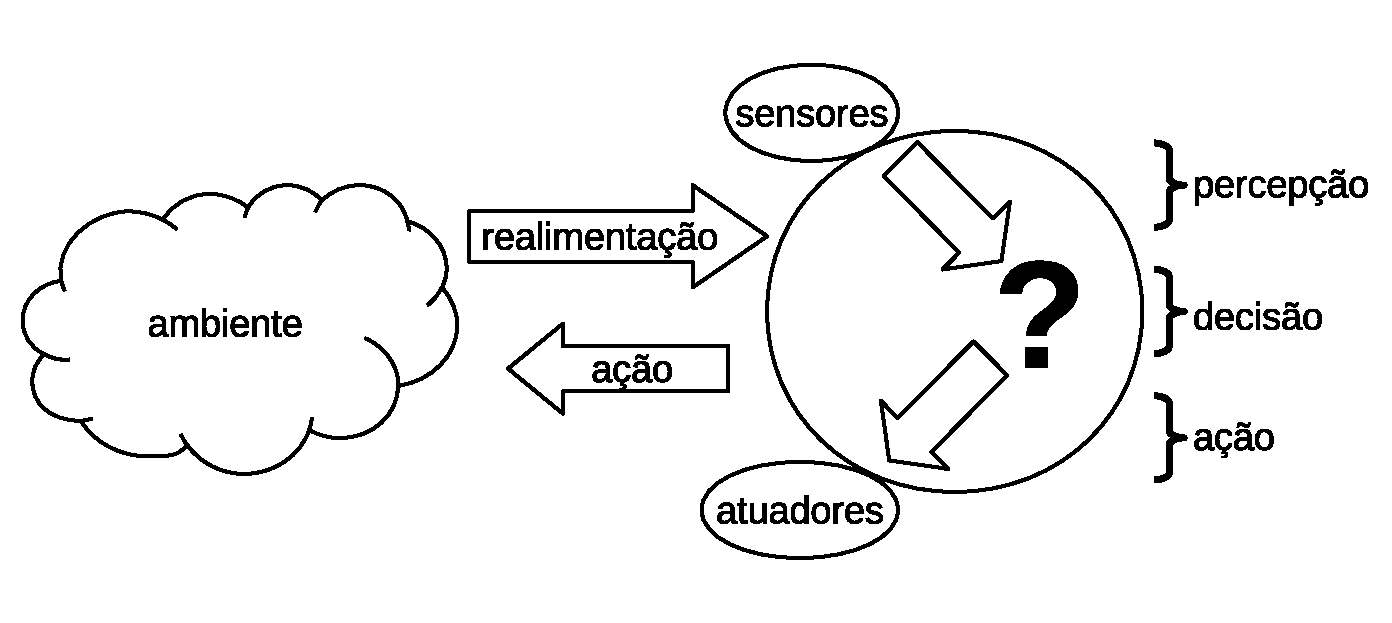
\includegraphics[width=3.0in]{Figuras/ambiente_agente.eps}
    \caption{\label{fig:ambiente_multiagente}Representação esquemática de um agente interagindo com seu ambiente.}
\end{figure}

\section{Padrões FIPA}

A comunicação ocupa um papel central em qualquer MAS. Além disso, para que dois agentes possam se comunicar é necessário que estes agentes entendam as mensagens transmitidas e recebidas. Com o intuito de padronizar o desenvolvimento de MAS interoperáveis, o Institute of Electrical and Electronics Engineers (IEEE) decidiu criar uma organização para cuidar de todos os detalhes relacionados ao desenvolvimento de MAS, e decidiu chamá-la de Foundation for Intelligent Phisical Agents (FIPA), que está vinculada à Sociedade de Computação do IEEE.

A FIPA tem por objetivo central definir padrões para tecnologias baseadas em sistemas multiagentes, proporcionando interoperabilidade entre os MAS e outras tecnologias [41]. A FIPA foi originalmente fundada em 1996 por um grupo de organizações acadêmicas e industriais que tinha como objetivo definir uma série de padrões e especificações que permitissem a usabilidade desses sistemas em uma ampla gama de aplicações [29].

A FIPA define padrões relacionados a três questões centrais em MAS: comunicação entre agentes, gerenciamento de agentes, e arquitetura dos agentes. Na \autoref{fig:plataformaFIPA} são mostrados os componentes que compõem uma plataforma de sistemas multiagentes definida pela FIPA.

\begin{figure}[htb]
    \centering
    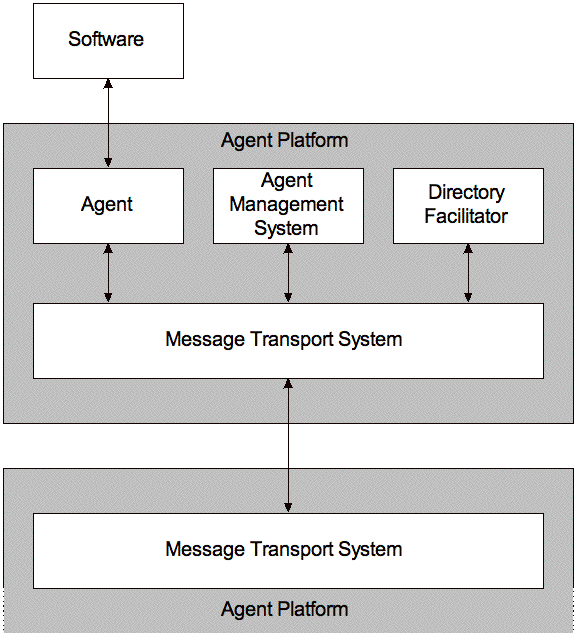
\includegraphics[width=2.0in]{Figuras/plataforma.png}
    \caption{\label{fig:plataformaFIPA}Plataforma de Sistemas Multiagentes definida pela FIPA}
\end{figure}

\section{Desenvolvimento da Plataforma}

De acordo com [29], essencialmente, um framework para o desenvolvimento de MAS deve oferecer três funcionalidades:
Uma biblioteca para a construção de agentes que implemente os padrões de interoperabilidade definidos pela FIPA;
Um ambiente de execução distribuído para que os agentes possam se comunicar e realizar suas atividades, mesmo estando em diferentes máquinas ou plataformas;
Um ambiente gráfico ou em linha de código que permita o monitoramento e controle das atividades dos agentes em execução.

Essas funcionalidades foram criadas para compor um framework de desenvolvimento de MAS em Python. O framework chama-se PADE e foi contruído utilizando as ferramentas disponíveis no Twisted, uma biblioteca escrita em Python utilizada para implementação de sistemas distribuídos. Na \autoref{fig:pade_geral} é mostrada a arquitetura dos módulos PADE construídos no topo das camadas Python/Twisted, dando suporte às aplicações multiagentes desenvolvidas e executadas utilizando suas bibliotecas e ambiente de execução, respectivamente.

\begin{figure}[htb]
    \centering
    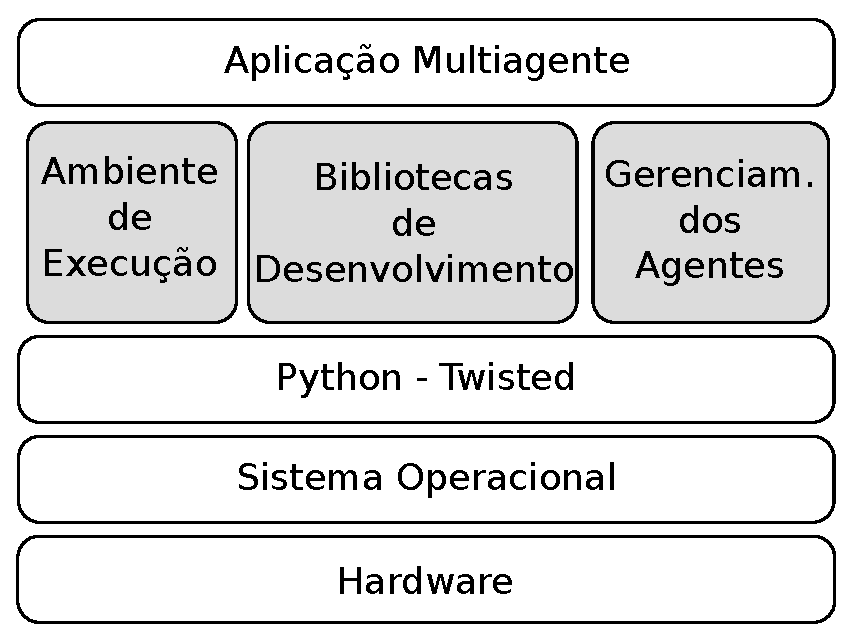
\includegraphics[width=1.8in]{Figuras/pade-visao-geral.eps}
    \caption{\label{fig:pade_geral} Arquitetura PADE}
\end{figure}


 PADE oferece os seguintes recursos em sua biblioteca para desenvolvimento de sistemas multiagentes:

 \begin{itemize}
   \item Abstração para construção de agentes e seus comportamentos utilizando conceitos de orientação a objetos;
  \item Módulo para inicialização do ambiente de execução de agentes, inteiramente em código Python;  
  \item Módulo para construção e tratamento de mensagens no padrão FIPA-ACL;
  \item Módulo para filtragem de mensagens;
  \item Módulo para a implementação dos protocolos definidos pela FIPA;
  \item Módulo para implementação de comportamentos cíclicos e temporais;
  \item Módulo para interação com banco de dados;
  \item Possibilidade de envio de objetos serializados como conteúdo das mensagens FIPA-ACL;
 \end{itemize}

Além dessas funcionalidades, o PADE é de fácil instalação e configuração, multiplataforma, podendo ser instalado e utilizado em hardwares embarcados que executam sistema operacional Linux, como Raspberry Pi e BeagleBone Black, bem como sistema operacional Windows.

Além disso, como a linguagem de programação Python foi a utilizada para o desenvolvimento da plataforma muitas funcionalidades estão incluídas em suas bibliotecas padrões e nos inúmeros projetos que são desenvolvidos pela comunidade. Python possui algumas características importantes, que estimularam sua utilização e que contribuem para que projetos de sistemas de automação distribuídos sejam bem sucedidos, como por exemplo, ser software livre, multiplataforma, ter sintaxe fácil e concisa, além de estar sendo adotado por uma grande parcela da comunidade científica, muito por conta dos módulos numpy e scipy que implementam facilidades de manipulação de matrizes e algoritmos de uso geral como inversão de matrizes, cálculo de autovalores ou transformada de Fourier.

\subsection{Framework Twisted}

Twisted é um mecanismo de rede, assíncrono, baseado em eventos e escrito em Python. Twisted tem suporte aos protocolos mais comuns das camadas de transporte e aplicação da internet como: TCP, UDP, HTTP, SSH, IMAP, FTP, entre outros. Twisted implementa versões de cliente e servidor destes protocolos, assim como oferece ferramentas que facilitam sua manipulação e configuração [43].

Twisted também oferece ferramentas de baixo nível para que protocolos genéricos sejam implementados na camada de aplicação de maneira fácil e rápida. Foram estas as ferramentas utilizadas no desenvolvimento do framework PADE.

\subsubsection{Programação Assíncrona Orientada a Evnetos} 

Quando sistemas distribuídos são desenvolvidos baseados no paradigma de programação síncrona, existem duas escolhas para o desenvolvedor: não tratar requisições externas enquanto um evento é processado ou desenvolver a aplicação fazendo uso de threads, que por vezes pode introduzir complexidade extra ao software.

No paradigma de programação assíncrona, o software desenvolvido continua podendo receber e tratar múltiplas conexões, mesmo enquanto está processando eventos anteriores, sem a necessidade de ter que controlar threads. Dessa forma, o paradigma de programação assíncrona contrasta com os outros dois possíveis tipos de programação, o single-thread síncrono e o multi-thread [43]:

Single-thread síncrono: Neste paradigma de programação as ações realizadas pelo programa são executadas de forma serial. Se alguma tarefa for bloqueada, todas as outras tarefas do programa precisarão esperar o encerramento desta tarefa para que possam ser executadas. Este tipo de programação é o mais simples de ser implementado, mas para alguns casos pode sofrer com problemas de lentidão, que tornaria este tipo de implementação impraticável.
Multi-thread: Neste paradigma de programação as tarefas de um determinado programa são executadas paralelamente por threads de controle diferentes. Isto permite que o software continue tratando eventos, mesmo com o bloqueio de uma determinada tarefa. No entanto, construir blocos de código que consumam recursos paralelamente de hardware pode não ser uma tarefa muito simples, o que aumenta bastante a complexidade do código a ser escrito.

No paradigma single-thread assíncrono as tarefas de um determinado programa são executadas intercaladamente em um único thread de controle. Esse paradigma combina as vantagens de execução de programas com múltiplas threads, com a facilidade de implementação de um programa de thread única.

Na \autoref{fig:paradigs} é ilustrada a execução de um programa que precisa executar três tarefas, utilizando cada um dos paradigmas de programação citados.

\begin{figure}[htb]
    \begin{center}
        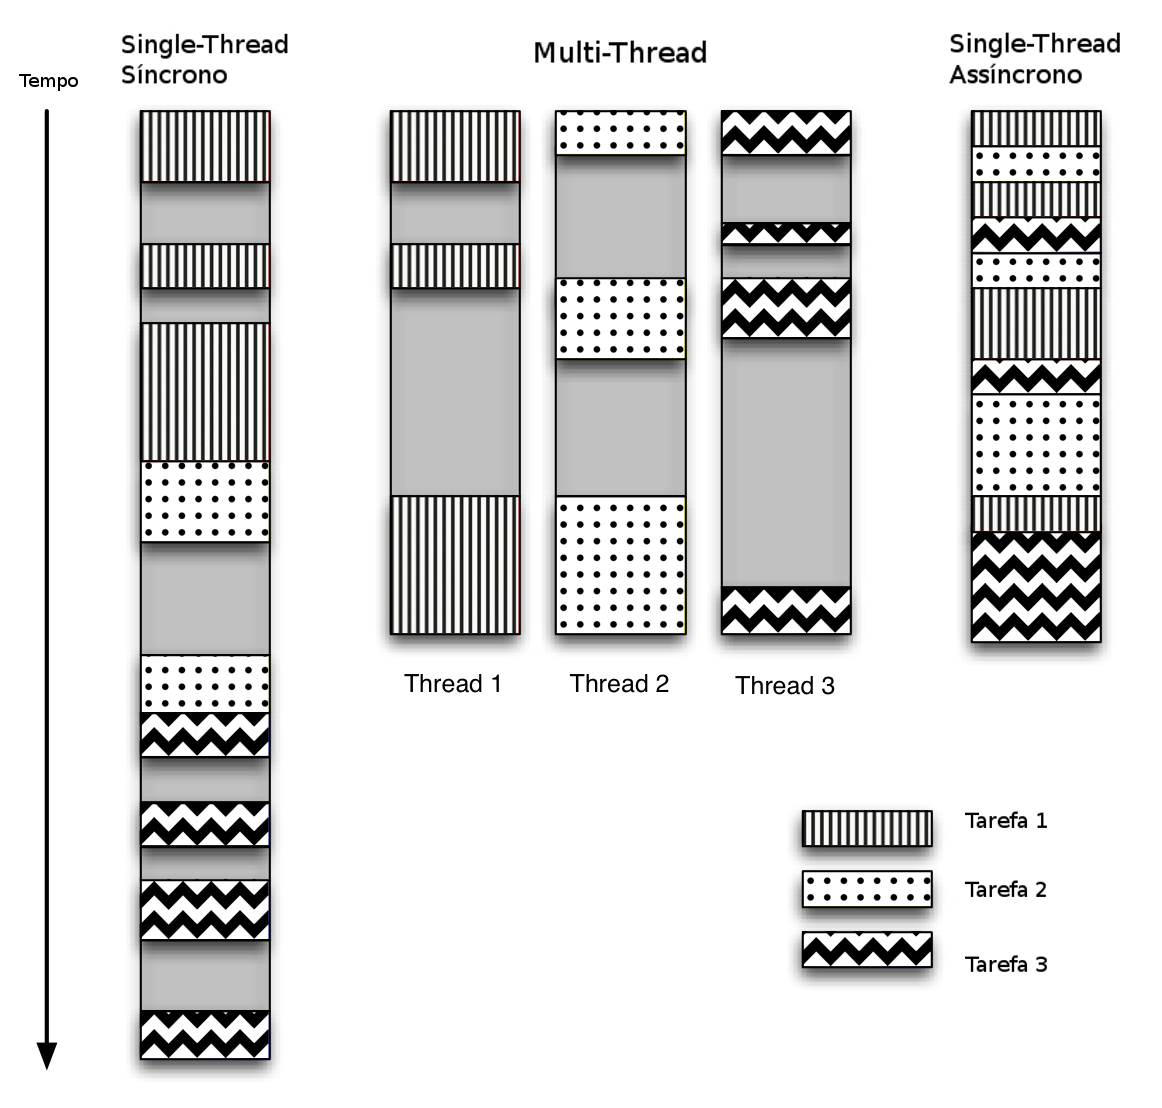
\includegraphics[width=2.2in]{Figuras/paradigmas.png}
        \caption{\label{fig:paradigs}Paradigmas de programação}
    \end{center}
\end{figure}

Já o conceito de programação orientada a eventos (assíncrono), refere-se à característica do fluxo do programa ser determinado por eventos externos. Esse tipo de paradigma utiliza sempre um loop de eventos reactor loop assim como métodos que são chamados quando um evento acontece callbacks.  Na \autoref{fig:reactor} é mostrada uma representação do loop de eventos Twisted e da chamada de uma callback quando um evento é processado.

\begin{figure}[htb]
    \centering
    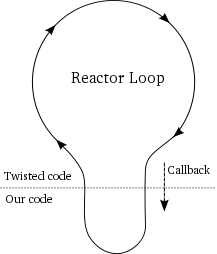
\includegraphics[width=1.2in]{Figuras/reactor-callback.png}
    \caption{\label{fig:reactor} \textit{Loop} de eventos do Twisted e chamada de uma \textit{callback}.}
\end{figure}

\subsubsection{Componetes Básicos do Twisted}

O Twisted possui alguns componentes básicos que fazem parte de sua arquitetura de funcionamento. Para desenvolver qualquer aplicação com Twisted é necessário conhecer e compreender as funcionalidades desses componentes. Os principais componentes do Twisted são [43]:

Reactor: É o núcleo do Twisted, chamado também de loop principal. Este loop supervisiona os eventos que decorrem de chamadas de protocolos de rede, de temporização ou de alteração na estrutura do sistema de arquivos. Na ocorrência de qualquer um desses eventos, o reactor os direciona para o método responsável por tratá-los;

Transport: Este componente fornece as interfaces necessárias para se estabelecer conexão entre dois pontos comunicantes em rede;

Protocols: Twisted fornece interfaces que implementam como eventos relacionados a diversos protocolos da camada de aplicação devem ser tratados, como por exemplo, chamadas HTTP, Telnet, DNP, FTP, IMAP, entre outros. Mas, também, Twisted oferece as ferramentas necessárias para que protocolos customizados sejam construídos;

Protocol Factories: Twisted instancia um objeto Protoco sempre que, por exemplo, uma nova conexão é realizada com um servidor. No entanto, esta instância é perdida assim que a conexão é encerrada, dessa forma todas as informações desta conexão são perdidas. Com o intuito de armazenar informações permanentes no protocolo, Twisted implementa o componente Protocol Factories de modo que informações pertinentes, como, por exemplo, quantos clientes estão conectados no servidor, sejam mantidas, mesmo depois que estas conexões sejam encerradas.

Na \autoref{fig:agentes_twisted} são mostrados os componentes do Twisted, que associados constituem o conceito de um agente na plataforma PADE. Conforme pode ser visto, um agente pode ser representado como a associação de:
\begin{itemize}
  \item uma instância da classe ProtocolFactory;
  \item várias instâncias da classe Protocol, uma para cada nova conexão estabelecidada com o agente;
  \item várias instâncias da classe Transport para abstrair a comunicação via rede com outos agentes;
  \item um loop de eventos, o Reactor Loop, que gerencia as solicitações recebidas pelo agente.
\end{itemize}

\begin{figure}[htb]
    \centering
    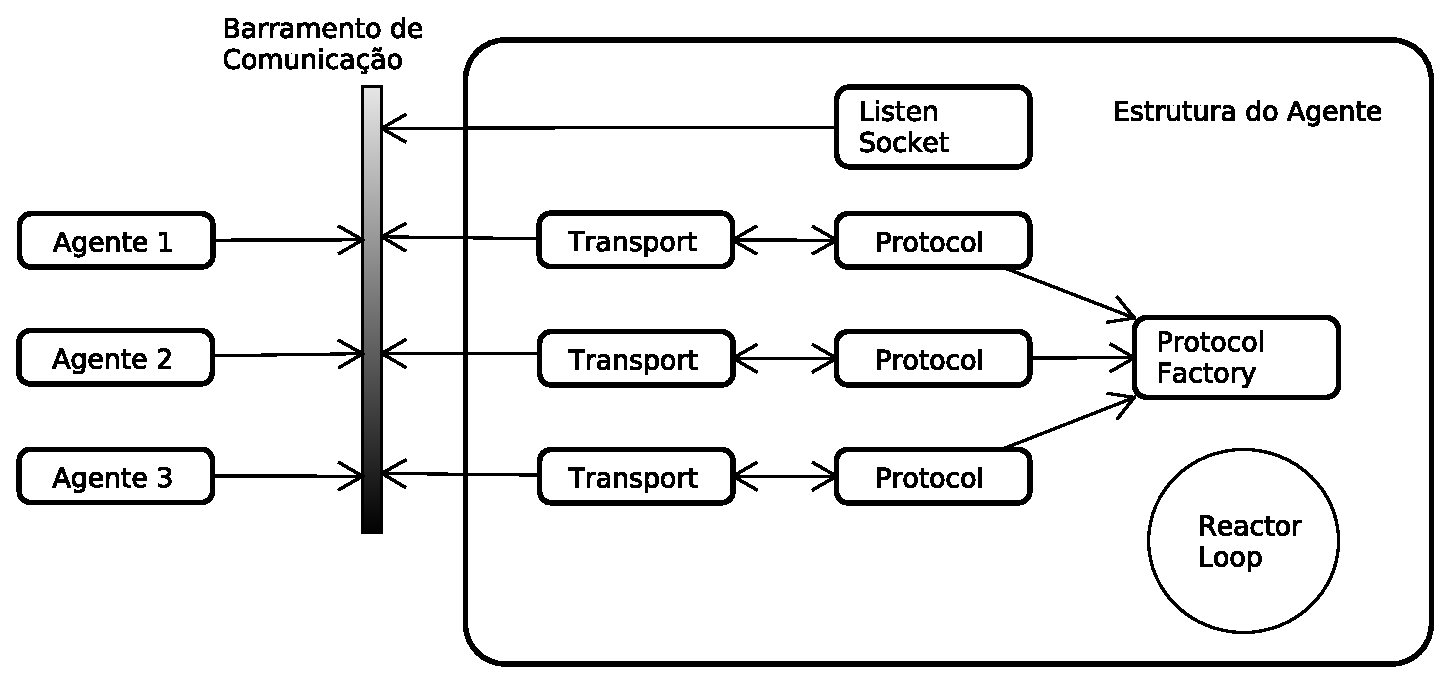
\includegraphics[width=3.0in]{Figuras/agente_twisted.eps}
    
    \caption{\label{fig:agentes_twisted} Concepção de um agente utilizando os módulos do Twisted.}
    % \legend{Fonte: Adaptado de ---.}
\end{figure}

\subsection{Python Agent DEvelopment framework}

Nesta seção é mostrado o desenvolvimento de um framework para desenvolvimento de sistemas multiagentes: o Python Agent DEvelopemnt framework (PADE), que permite a implementação, execução e monitoramento de um MAS em ambiente distribuído. Entre muitas vantagens PADE possui uma abordagem clara e fácil fazendo uso da principal funcionalidade do Python: simplicidade, além de prover acesso facilitado entre agentes sendo executados em diferentes dispositivos.

Utilizando como base de implementação o framework Twisted, foi desenvolvido o PADE, um framework para desenvolvimento, gerenciamento e execução de MAS em Python. O PADE segue alguns dos padrões estabelecidos pela FIPA, que visam interoperabilidade entre MAS desenvolvidos em diferentes plataformas, buscando sempre uma abordagem de comunicação mais direta e objetiva.

\subsubsection{Estrutura de Arquivos do PADE}

O framework PADE é composto por sete módulos principais que agrupam suas funcionalidades. A seguir a descrição de cada um dos módulos PADE:

\begin{itemize}
  \item acl: implementa alguns dos padrões FIPA de comunicação entre agentes, como por exemplo a possibilidade de composição de mensagens no padrão FIPA-ACL, definidos em [44]–[46].
  \item behaviours: implementa alguns dos comportamentos e protocolos definidos e padronizados pela FIPA para execução pelos agentes, [47]–[49];
  \item core: principal módulo do PADE, onde são implementados os algoritmos de cliente e servidor dos agentes por meio do framework Twisted. É nesse módulo que estão implementadas as funções de execução de agentes definidos pelo usuário e dos agentes padrões: AMS e Sniffer, definidos em [50];
  \item db: módulo que implementa a comunicação do núcleo do framework PADE com um banco de dados. Por meio deste módulo o framework pode, por exemplo, armazenar todas as mensagens trocadas pelos agentes;
  \item gui: onde estão implementadas as classes que definem a interface gráfica do AMS;
  \item misc: módulo onde estão implementadas algumas funcionalidades de uso geral, como, por exemplo, exibir mensagens de forma padronizada na tela;
  \item tests: módulo de testes, a ser implementado futuramente.
\end{itemize}

\subsubsection{Filosofia de Execução dos Agentes no Framework PADE} 

O núcleo do framework PADE consiste na funcionalidade de execução dos agentes e está descrito na \autoref{fig:uml_pade} em forma de diagrama de classes do padrão UML. Na \autoref{fig:uml_pade} é possível visualizar a classe Agent e suas relações com as demais classes no módulo core.

\begin{figure}[!htb]
    \centering
    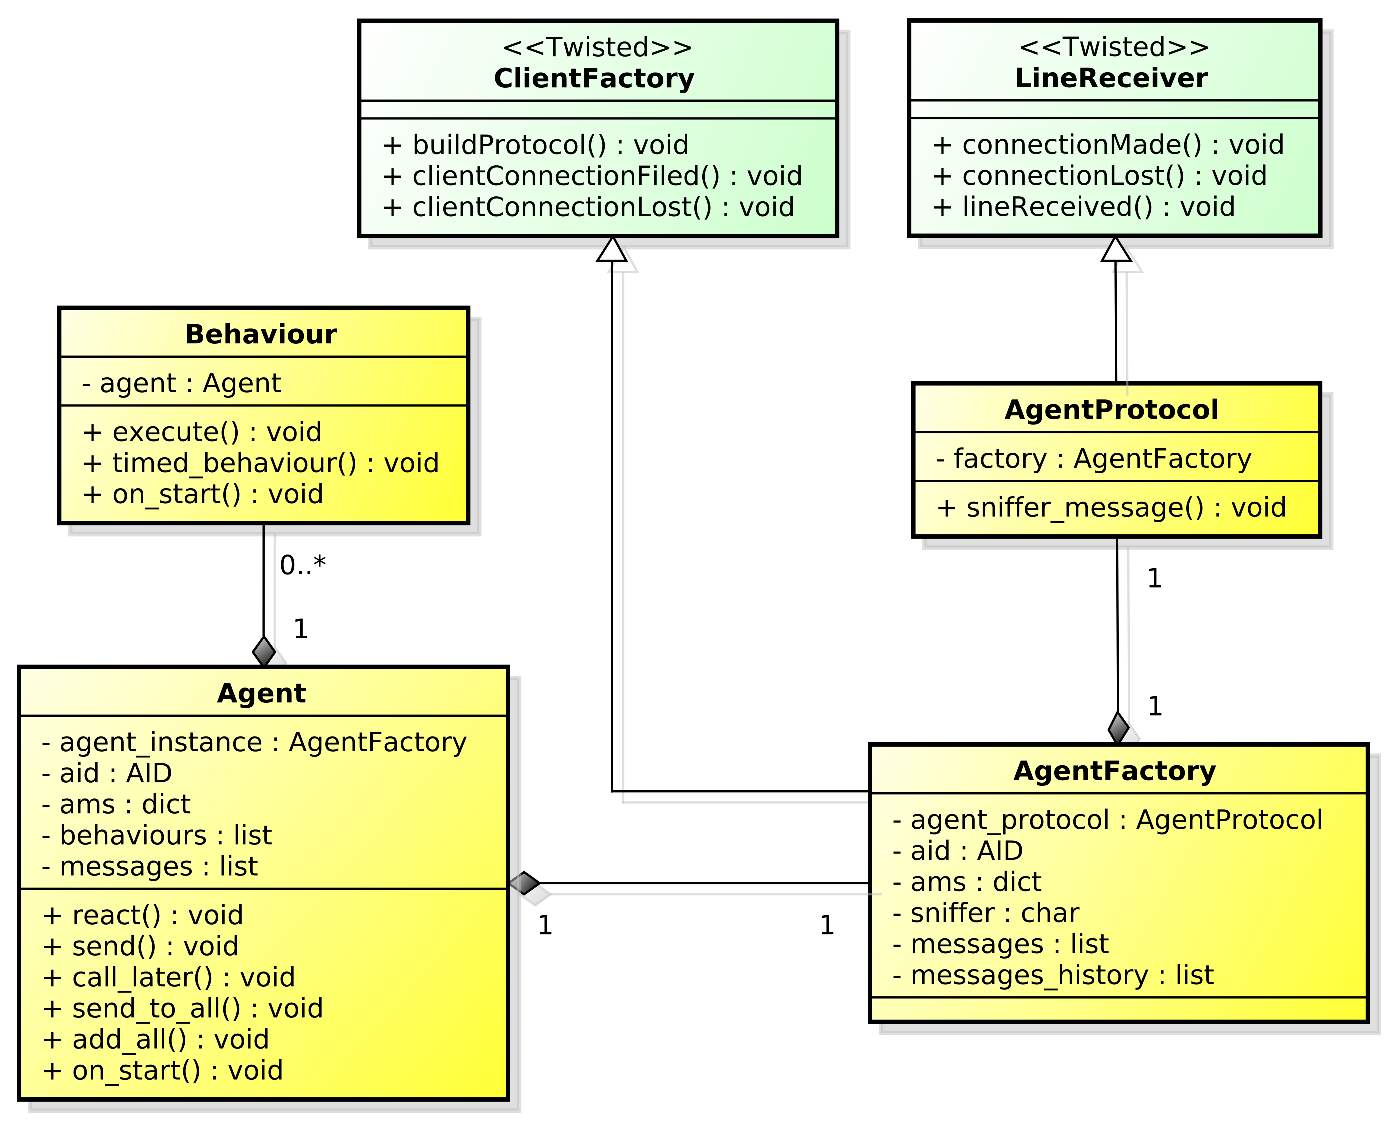
\includegraphics[width=3.0in]{Figuras/Core.eps}
    \caption{\label{fig:uml_pade} Estrutura de classes do framework PADE no padrão UML.}
\end{figure}

Todo agente desenvolvido com os módulos disponibilizados pelo framework deve herdar da classe Agent. Esta classe implementa um protocolo definido pelas bibliotecas do Twisted, e representados na Fig. 7 por meio das classes AgentProtocol e AgentFactory. Essa implementação permite que um agente comporte-se hora como cliente, hora como servidor, ou seja, um agente é um nó comunicante na rede, que pode inciar uma troca de mensagens, mas que também está disponível para responder solicitações de outros nós da rede, bastando que para isso os agentes conheçam os endereços uns dos outros.

Um agente na plataforma é identificado pelo seu AID (Agent IDentifier) que tem a seguinte composição:  nome local@endereçoIPdoagente:porta. Um exemplo de AID para um agente de nome alimentador\_21I5 que é executado na máquina de IP 192.168.1.2 na porta 5002, seria: alimentador\_21I5@192.168.1.2:5001.

\subsubsection{O Agente AMS}

O Agent Management System (AMS) desempenha função muito importante para a plataforma de MAS e de acordo com o padrão [50], que define as características e atribuições do AMS, é mandatória a presença de um gerenciador na plataforma.

No PADE, o AMS exerce funções de controle e supervisão e mantém uma tabela que contém os identificadores dos agentes. De acordo ainda com a FIPA, os agentes precisam registrar-se no AMS para adquirirem um identificador válido, sendo assim capazes de se comunicar com outros agentes.

No PADE, o AMS é um agente, e necessariamente deve ser o primeiro agente a ser lançado, já que os outros precisam do AMS para se cadastrar. 

Cada agente lançado na plataforma deve enviar mensagem ao agente AMS identificando-se e, assim, ficando visível aos demais agentes. O processo de um agente que solicita identificação e do AMS que recebe e analisa o pedido pode ser representado por meio de um diagrama de atividades conforme mostrado na \autoref{fig:identificacao}.

\begin{figure}[!htb]
    \centering
    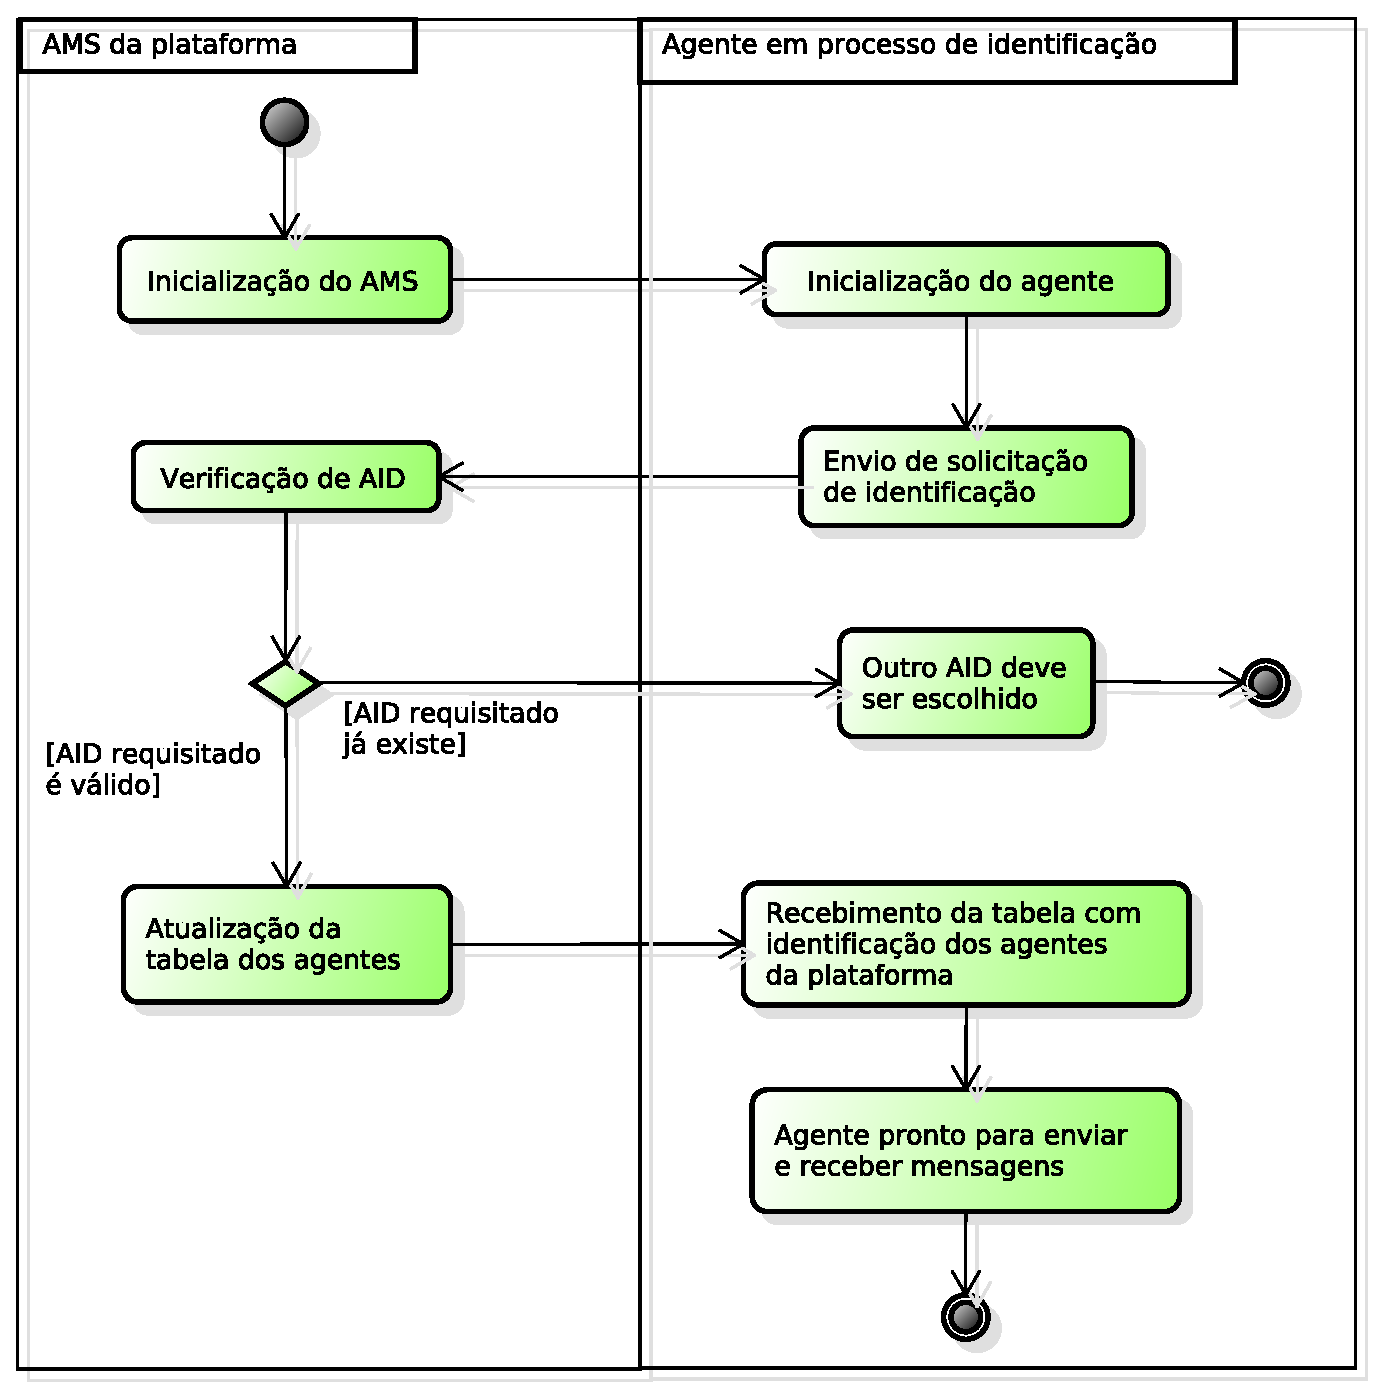
\includegraphics[width=3.2in]{Figuras/identificacao.eps}
    \caption{\label{fig:identificacao} Diagramas atividades do processo de identificação no PADE.}
\end{figure}

O diagrama mostrado na \autoref{fig:identificacao} descreve os comportamentos de:

\begin{itemize}
  \item solicitação de identificação: o agente que acabou de conectar-se à rede de comunicação envia seu AID ao AMS solicitando identificação e permissão para entrar na plataforma de agentes;
  \item análise de solicitação: o agente AMS recebe a solicitação do agente e verifica se o AID enviado já existe entre os AID dos agentes ativos na plataforma. Se nenhum dos agentes ativos estiver cadastrado com o AID solicitado, então o AMS envia mensagem de autorização para entrada do agente.
  \item resposta da solicitação: caso tenha seu pedido aceito, o agente recebe uma tabela com os endereços de todos os agentes presentes na plataforma e pode comunicar-se com cada um deles. Caso tenha seu pedido de identificação negado, o agente deve enviar uma nova proposta com AID diferente para o AMS.

\end{itemize}

No PADE, assim como o AMS, cada agente possui uma tabela com o nome e o endereço de cada agente em execução na plataforma. Essa tabela é distribuída e atualizada pelo AMS sempre que um agente entra ou sai da plataforma. Essa situação pode ficar bem clara por meio de um exemplo.

Os agentes Bob, Eva e Alice, inicialmente estão fora da plataforma PADE. Primeiro o agente Bob é executado. Bob se registra junto ao AMS que valida seu AID. Como não existe nenhum outro agente em execução na plataforma, nenhuma tabela é criada ou atualizada. Em seguida o agente Alice entra em execução registrando-se junto ao AMS, que valida seu AID, atualiza sua tabela de agentes ativos e distribui esta tabela aos demais agentes da rede, no caso para o agente Bob. Da mesma forma, o agente Eva também se registra junto ao AMS, que atualiza as tabelas de todos os agentes (Bob e Alice) com o novo agente disponível para comunicação. Essa situação é mostrada na \autoref{fig:diag_seq_1}.

\begin{figure}[!htb]
    \centering
    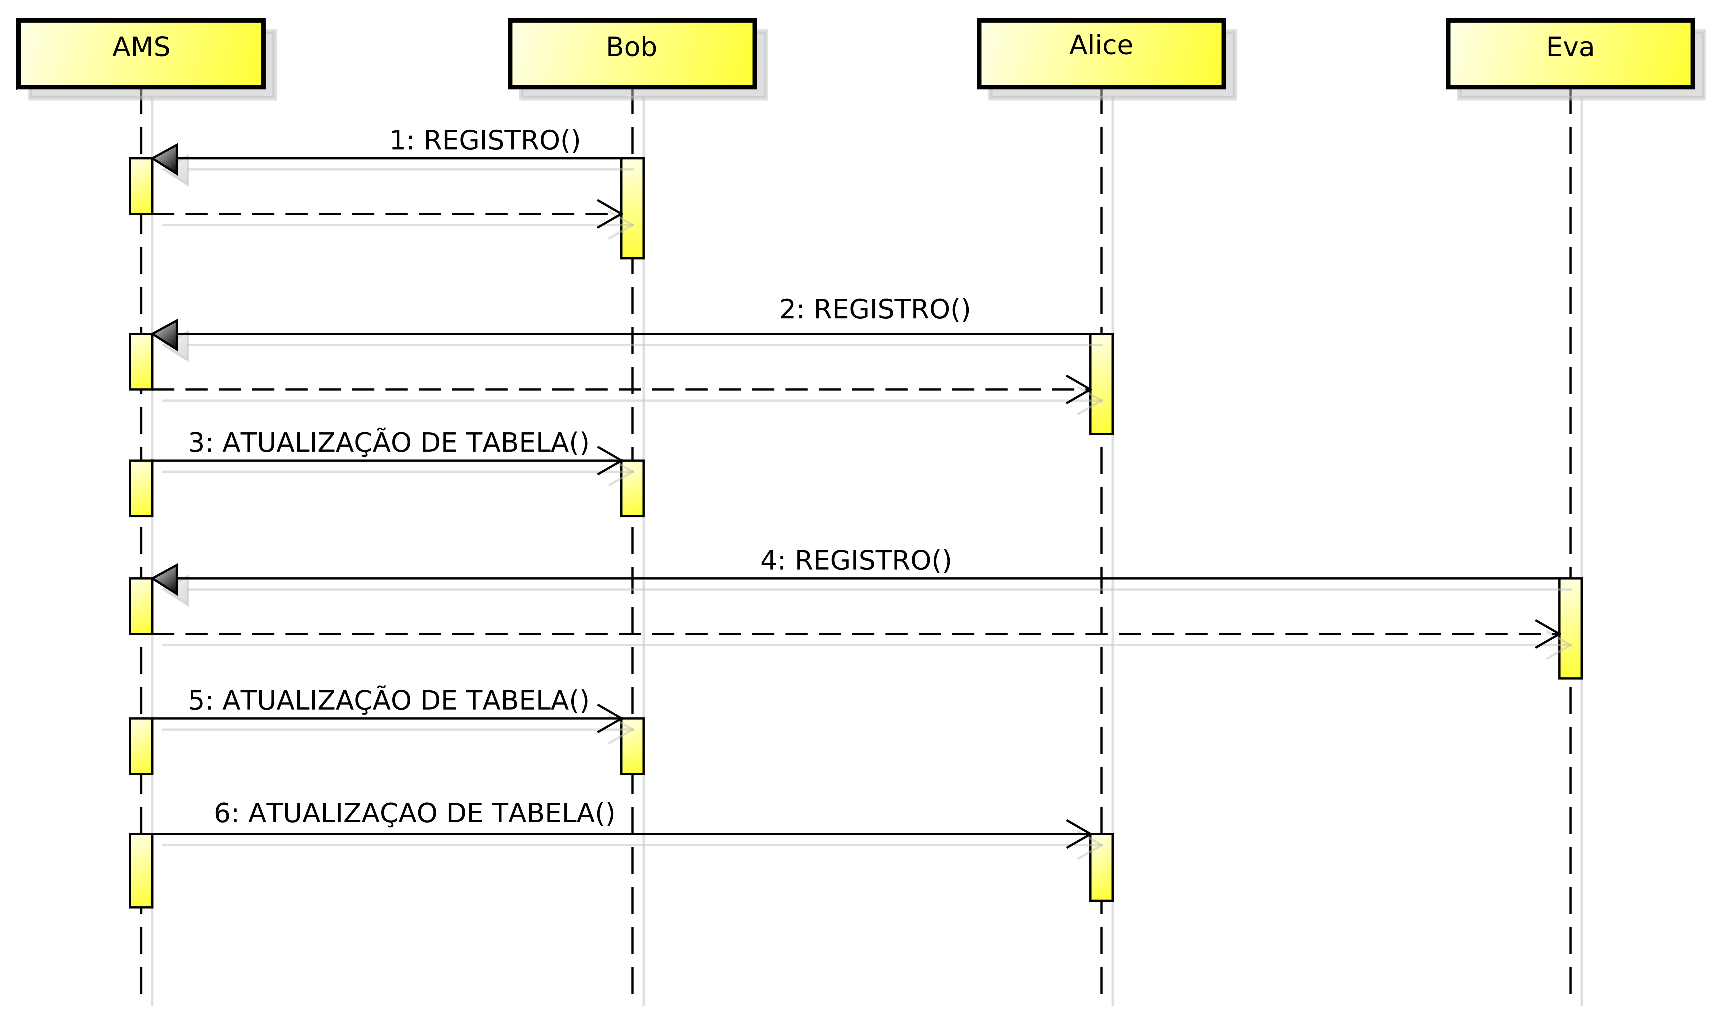
\includegraphics[width=3.2in]{Figuras/alice_bob_eva.eps}
    \caption{\label{fig:diag_seq_1}Registro e atualização de tabela de agentes.}
\end{figure}

Dessa forma quando um agente deseja se comunicar com outro, busca em sua própria tabela o endereço do agente destino, sem precisar perguntar o endereço ao agente AMS, e mesmo que o agente AMS seja desativado, os agentes ainda serão capazes de se comunicar, pois possuem a tabela de endereços dos agentes permanecentes na rede.

Logicamente sem a presença de um agente AMS na plataforma, as funções de supervisão, registro e controle ficam desprovidas pela plataforma. Mas a comunicação dos agentes que já estavam na plataforma continua possível, o que em muitos casos pode ser útil, no entanto esta deve ser uma situação temporária, uma vez que depois que o agente AMS é desativado, a tabela de agentes não poderá mais ser atualizada.

\subsubsection{O Agente Snnifer}

Outro componente muito útil em uma plataforma multiagente é o agente Sniffer. No PADE, o agente Sniffer tem a função de enviar mensagens periódicas aos agentes para realizar testes de conexão. Caso o agente não responda à mensagem, é informado ao AMS que o agente não está mais na plataforma e, assim, a tabela dos outros agentes é atualizada.

Outra função que é executada pelo agente Sniffer é o registro das conversas realizadas pelos agentes. Essas mensagens tanto podem ser armazendas em um arquivo de log como podem ser exibidas em uma interface gráfica. Na  \autoref{fig:guis} é mostrada a janela principal da interface gráfica do agente Sniffer, que exibe na coluna da esquerda todos os agentes que estão ativos e que possuem cadastro junto ao AMS e na coluna da direita as mensagens recebidas pelo agente selecionado, juntamente com a janela secundária da interface do agente Sniffer, que é lançada ao selecionar alguma das mensagens exibidas na janela principal, onde são mostrados todos os campos da mensagem no padrão ACLMessage recebida pelo agente selecionado.

\begin{figure*}[!htb]
        \centering
        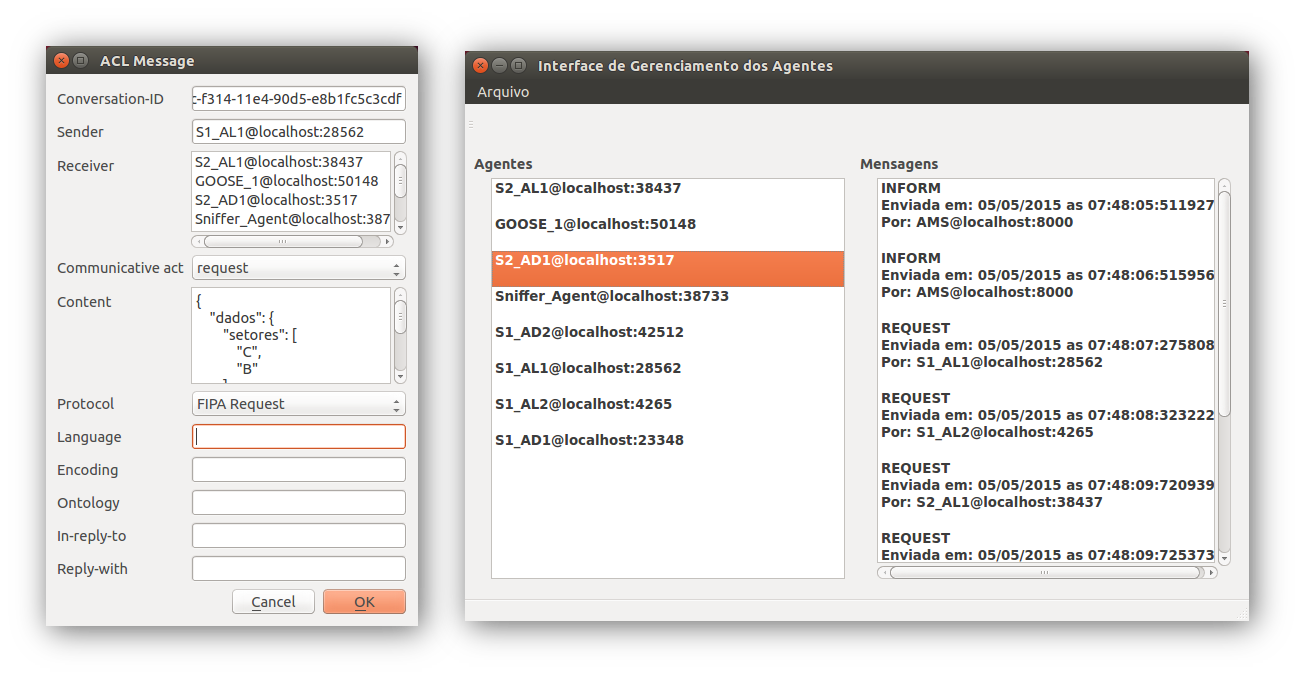
\includegraphics[width=5.0in]{Figuras/guis.png}
        \caption{\label{fig:guis} Interface gráfica de registro de mensagens trocadas entre agentes no PADE.}
\end{figure*} 

\subsubsection{Estrutura de um Agente Modelado no PADE}

A estrura de código de um agente modelado por meio do framework PADE é bem simples e tem um padrão definido. Este padrão consiste em:

classes que herdam de um comportamento/protocolo disponibilizado pelo PADE;
uma classe que herda da classe Agent.

Dessa forma, um arquivo que modele um agente no PADE sempre terá uma única classe que representa a instância do agente, e quantas classes forem necessárias para representar instâncias dos comportamentos definidos para os agentes.

Por exemplo, para implementar um comportamento do tipo Contractnet Iniciante no PADE, o diagrama de classes UML mostrado na \autoref{fig:agente_alimentador_uml} pode ser utilizado. No diagrama UML é possível observar que a classe AgenteAlimentador herda da classe Agent todas as características necessárias para que o agente possa ser executado, identificado e em seguida consiga estabelecer comunicação com os demais. A classe ContractNetComport herda da classe ContractNet todos os métodos necessários para que o protocolo FIPA ContractNet seja implementado, podendo ser do tipo iniciante ou participante. Por fim, existe uma associação do tipo composição entre as classes AgenteAlimentador e ContractNetComport que indica que um objeto do tipo AgenteAlimentador pode conter um ou vários objetos ContractNetComport.

\begin{figure}[!htb]
    \centering
    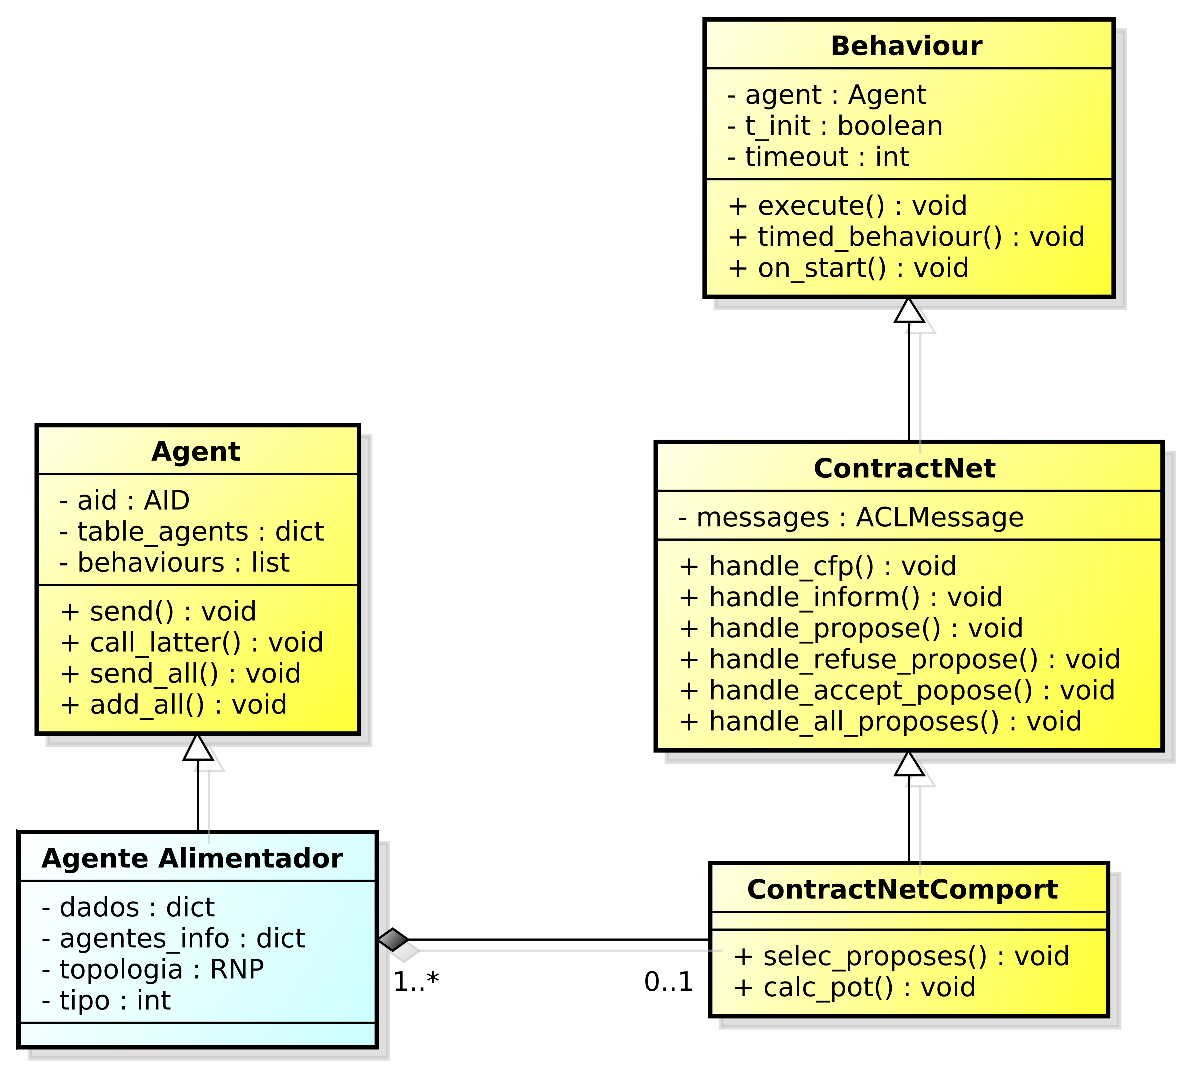
\includegraphics[width=3.2in]{Figuras/agente_alimentador.eps}
    \caption{\label{fig:agente_alimentador_uml} Diagrama de classes UML de um agente que tem um comportamento FIPA ContractNet associado.}
\end{figure}

\section{Caso Teste}

Nesta sessão será apresentada a utilização do framework PADE para o desenvolvimento de um sistema multiagente de recomposição automática de alimentadores da rede elétrica de distribuição. O sistema de recomposição deve ser capaz de, na ocorrência de uma falta, identificar o setor faltoso, isolá-lo do restante da rede e recompor os setores desenergizados, mas que não possuem defeito. Isso pode ser feito por que existem chaves normalmente fechadas (NF) ao longo da rede que são utilizadas para isolar os setores defeituosos e chaves normalmente abertas (NA) entre alimentadores distintos que podem ser utilizadas para reenergizar o alimentador por outros caminhos.

O problema da recomposição da rede elétrica mediante a ocorrência de uma falta é tratado como um problema de otimização com múltiplos objetivos, conflitantes entre sí, pois é necessário maximizar o número de consumidores re-energizados, mas com o menor número de manobras possíveis e respeitando as restrições operacionais do sistema, como por exemplo, sobrecarga das fontes e dos condutores da rede.

Na \autoref{fig:rede_6_b} é mostrado um sistema elétrico simplificado com duas subestações S1 e S2. A subestação S1 possui dois alimentadores S1\_AL1, que alimenta os setores A, B, C e F e o alimentador S1\_AL2 que alimenta os setores G, H e I. Na subestação S2 existe apenas um alimenador, o S2\_AL1 que alimenta dos setores D e E. Na representação adotada, as chaves NF são as linhas contínuas entre os setores, já as chaves NA são representadas por linhas racejadas.

\begin{figure}[htb]
    \centering
    
    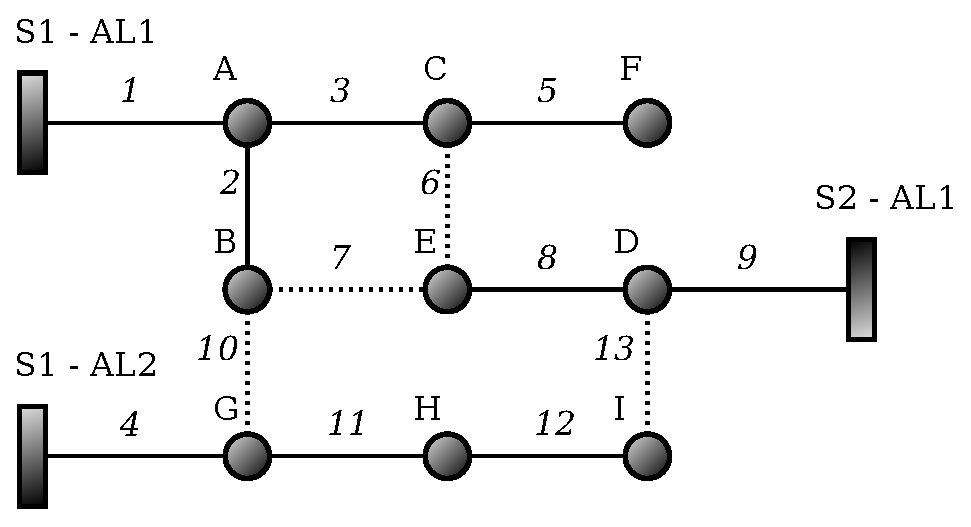
\includegraphics[width=2.5in]{Figuras/rede_estado_normal.eps}

    \caption{\label{fig:rede_6_b} Representação simplificada, baseada em grafos, dos setores, subestações e chaves da rede elétrica.}
    % \legend{Fonte: Própria do autor.}
\end{figure}

Após a ocorrência de uma falta permanente no setor A, a proteção irá atuar sob a chave 1 e desenergizar o alimentador S1\_AL1 por completo, deixando os setores B, C e F, que não têm problemas, desenergizados, conforme mostrado na \autoref{fig:teste_1_1}.

\begin{figure}[htb]
    \centering
    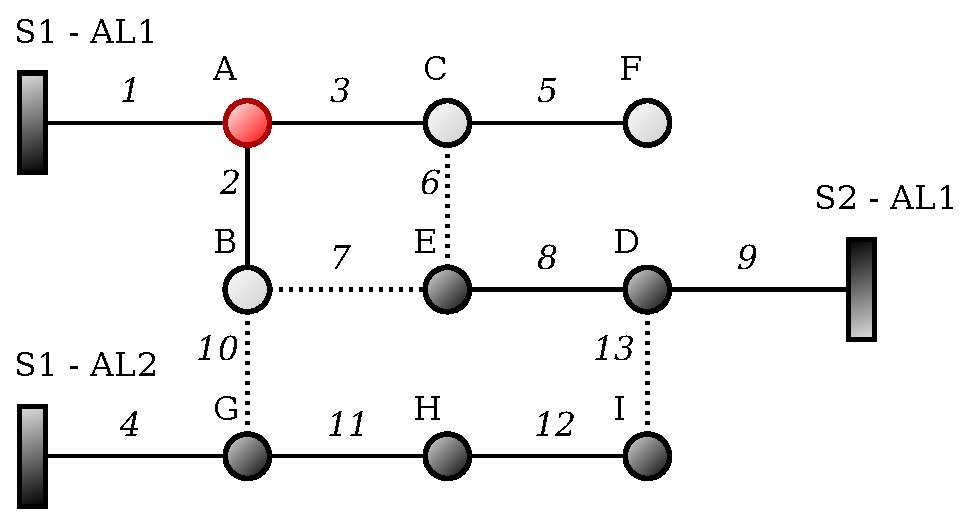
\includegraphics[width=2.5in]{Figuras/rede_curto_A.eps}
    \caption{\label{fig:teste_1_1} Atuação da proteção sobre a chave 1.}
\end{figure} 

Na ocorrência desses eventos o SMRA deve iniciar sua atuação, percebendo a ocorrência da falta elétrica, identificando o setor que está com defeito e imediatamente isolando-o do restante do sistema, por meio da abertura das chaves 2 e 3.

Quem realiza estes procedimentos iniciais de identificação do defeito, isolação do setor e comunicação com os dispositivos da rede é o agente Dispositivo, que depois de realizados estes procedimentos, comunica a ocorrência para o agente Alimentador que é o responsável por negociar com outros agentes a recomposição dos setores desenergizados, no caso B, C e F, além de analisar as restrições operacionais, ao executar um fluxo de carga de varredura direta-inversa sobre a topologia de rede proposta, só tomando alguma decisão após todos os critérios terem sido verificados e satisfeitos.  

A configuração final da recomposição pode ser visualizada na \autoref{fig:rede_recomposta}. 

\begin{figure}[htb]
    \centering
    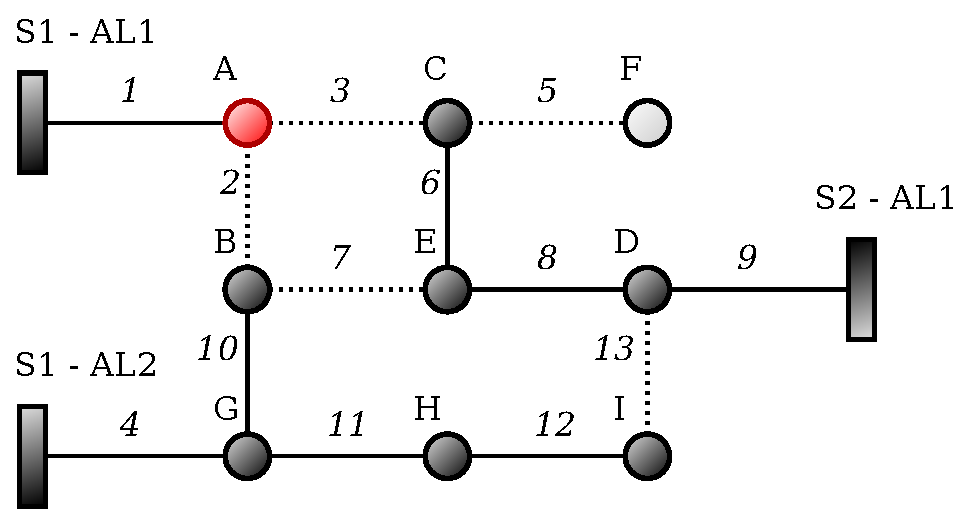
\includegraphics[width=2.5in]{Figuras/rede_recomposta.eps}
    \caption{\label{fig:rede_recomposta} Topologia da rede após a poda do setor F do alimentador S2-AL1.}
\end{figure}

Foram realizados testes e simulações com o SMRA desenvolvido utilizando o PADE. Foram utilizados na infraestrutura de testes três IED SEL-751 reais e comunicando via protocolos IEC 61850, interconectados por meio de um switch de rede também da SEL. Aos IED foi conectada uma mala de testes Conprove CE-6006 que simula o secundário do TC na ocorrência de uma falta na rede elétrica. Os agentes estão embarcados em computadores, além de hardwares Raspberry Pi e BeagleBone Black, conforme mostrado na arquitetura da \autoref{fig:top_teste}.

\begin{figure}[htb]
    \centering
    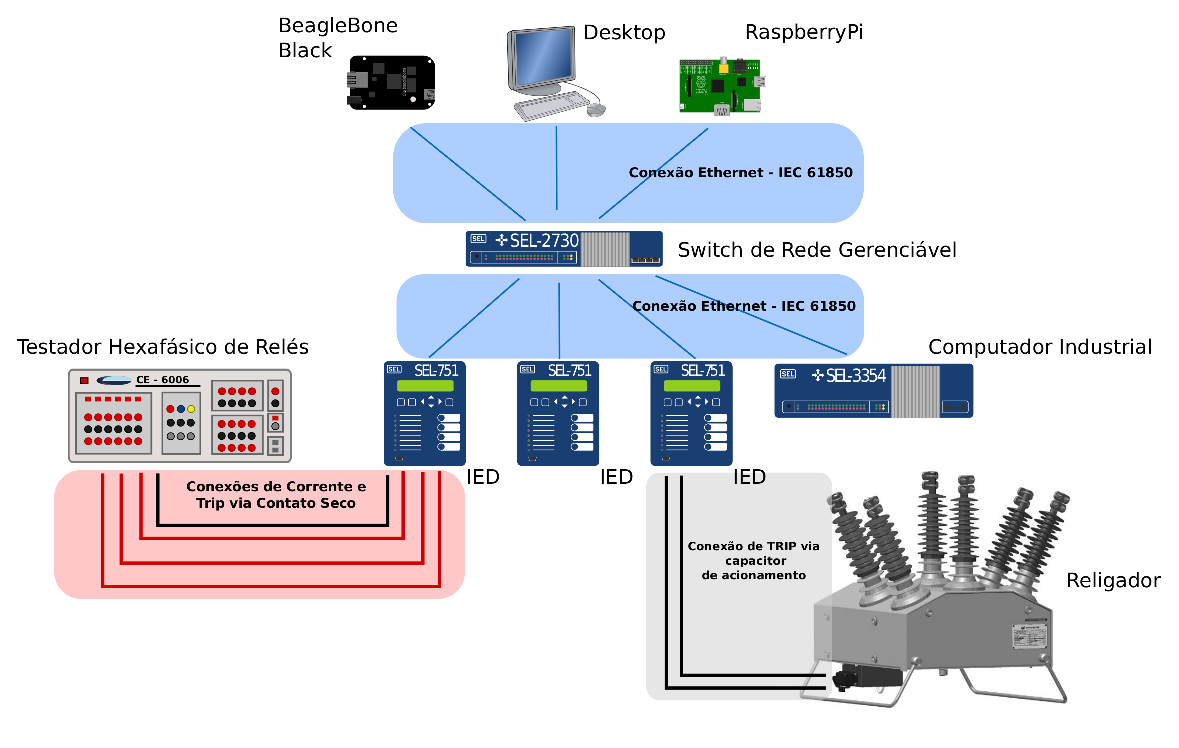
\includegraphics[width=3.0in]{Figuras/topologia_de_testes.eps}
    \caption{\label{fig:top_teste} Topologia física de testes do SMRA.}    
\end{figure}

Os agentes foram embarcados nos dispositivos computacionais (desktop, computador industrial, Raspberry Pi e BeagleBone Black) simulando um ambiente computacional distribuído e conectado via rede Ethernet por meio do switch SEL-2730, conforme mostrado na \autoref{fig:top_teste}. Na \autoref{tab:info_rede} são mostrados os dispositivos que são utilizados como contêineres de agentes e que fazem parte da infraestrutura de execução do SMRA, integrados em rede Ethernet e comunicando-se via protocolos estabelecidos pela FIPA. Os IED que também fazem parte da infraestrutura de comunicação Ethernet, podendo receber comandos por meio do protocolo MMS e publicar mensagens utilizando o protocolo GOOSE, também estão listados na \autoref{tab:info_rede}.

\begin{table}[htb]
    \centering
    \caption{\label{tab:info_rede} Dispositivos conectados em rede Ethernet para execução dos testes.}
    \begin{tabular}{p{1.0in}p{0.5in}p{1.0in}}
        \toprule
        Dispositivo & Função & Endereço IP \\[0.1in]
        \midrule
        \midrule
        Relé SEL 751 & DPC & 192.168.1.51 \\
        \midrule
        Relé SEL 751 & DPC & 192.168.1.52 \\
        \midrule
        Relé SEL 751 & DPC & 192.168.1.53 \\
        \midrule
        Laptop & CA & 192.168.1.10 \\
        \midrule
        Raspberry Pi & CA & 192.168.1.11 \\
        \midrule
        BeagleBone Black & CA & 192.168.1.12 \\
        \bottomrule
    \end{tabular}
    \\[0.1in]
    \legend{
    \begin{flushleft}
        Legenda:\\
        DPC: Dispositivo de proteção e controle.\\
        CA: Contêiner de agentes
    \end{flushleft}}
\end{table}

Levando em consideração a rede de testes mostrada na \autoref{fig:top_teste}, a plataforma de testes do SMRA possui três módulos de execução de agentes, sendo um por alimentador. Esta abordagem proporciona um ambiente de processamento distribuído para a execução dos agentes. Na \autoref{tab:agentes} são mostrados os agentes presentes em cada módulo de execução, assim como o alimentador associado e seu identificador, que funciona como um endereço vinculado aos hardwares listados na \autoref{tab:info_rede}.

\begin{table}[htb]
    \centering
    \caption{\label{tab:agentes} Agentes presentes na plataforma de testes do SMRA.}
    \begin{tabular}{p{0.8in}p{0.5in}p{1.0in}}
        \toprule
         \multicolumn{1}{c}{Alimentador} & \multicolumn{1}{c}{Agente} & \multicolumn{1}{c}{Tipo} \\[0.1in]
        \midrule
        \midrule
        \multirow{2}{1.0in}{S1-AL1} & S1\_AL1 & Alimentador \\
        & S1\_AD1 & Dipositivo \\
        \midrule
        \multirow{2}{1.0in}{S1-AL2} & S1\_AL2 & Alimentador \\
        & S1\_AD2 & Dispositivo \\
        \midrule
        \multirow{2}{1.0in}{S2-AL1} & S2\_AL1 & Alimentador \\
        & S2\_AD1 & Dispositivo \\
        \bottomrule
    \end{tabular}
    % \legend{Fonte: Própria do autor.}
\end{table}

\section{Conclusão}

PADE é um framework para desenvolvimento, execução e monitoramento de sistemas multiagentes desenvolvido em Python com base no framework Twisted para desenvolvimento de sistemas distribuídos assíncronos baseados em eventos. PADE é uma alternativa às plataformas de desenvolvimento e execução de agentes já existentes, possibilitando ao SMRA ser implementado em uma linguagem de programação moderna, com utilização do paradigma de orientação a objetos, de fácil aprendizado e com recursos para o desenvolvimento de sistemas distribuídos.

O PADE possui uma filosofia de comunicação distribuída com independência de agente gerenciador para manutenção da comunicação, além de poder ser executado em hardware embarcado com procesador ARM de 700 MHz de frequência e 512 MB de memória RAM. 

O PADE utiliza os aspectos recomendados pela FIPA na implementação de plataformas multiagentes, fazendo uso de uma abordagem direta e objetiva. Isso confere ao PADE a característica de simplicidade de implementação e de execução. Alguns dos aspectos disponibilizados pelo PADE para o desenvolvimento e execução de agentes, são:

\begin{itemize}
    \item Defição do padrão FIPA-ACL de mensagens entre agentes;
    \item Definição de protocolos definidos pela FIPA para comunicação entre agentes: FIPA-Request, FIPA-ContractNet, FIPA-Subscribe;
    \item Definição de uma estrutura de classes que organizam a implementação dos comportamentos dos agentes;
    \item interface gráfica para a visualização de troca de mensagens entre agentes;
    \item Execução dos agentes em um loop de eventos assíncrono de thread única;
    \item Plataforma de execução dos agentes em ambiente distribuído de comunicação.
\end{itemize}

O PADE foi testado e validado com uma topologia de agentes inteligentes que implementam um sistema de recomposição automática de alimentadores de distribuição de energia elétrica em um contexto de redes elétricas inteligentes. Os agentes implementados em PADE detectam ocorrências na rede elétrica, realizam cálculos de topologia e de carregamento elétrico, negociam potência entre sí e comandam equipamentos de controle e proteção no sistema elétrico via protocolos de comunicação estabelecidos pela norma IEC 61850.

Tudo isso mostra a flexibilidade e aplicabilidade da plataforma PADE no desenvolvimento de sistemas multiagentes para aplicações reais e com alto grau de confiabilidade e disponibilidade.


% use section* for acknowledgment
\section*{Agradecimentos}

Agradecemos ao CNPq e à Companhia Energética do Ceará pelo apoio e ao Departamento de Engenharia Elétrica da Universidade Federal do Ceará pelo suporte de laboratório.


% Can use something like this to put references on a page
% by themselves when using endfloat and the captionsoff option.
\ifCLASSOPTIONcaptionsoff
  \newpage
\fi



% trigger a \newpage just before the given reference
% number - used to balance the columns on the last page
% adjust value as needed - may need to be readjusted if
% the document is modified later
%\IEEEtriggeratref{8}
% The "triggered" command can be changed if desired:
%\IEEEtriggercmd{\enlargethispage{-5in}}

% references section

% can use a bibliography generated by BibTeX as a .bbl file
% BibTeX documentation can be easily obtained at:
% http://www.ctan.org/tex-archive/biblio/bibtex/contrib/doc/
% The IEEEtran BibTeX style support page is at:
% http://www.michaelshell.org/tex/ieeetran/bibtex/
%\bibliographystyle{IEEEtran}
% argument is your BibTeX string definitions and bibliography database(s)
%\bibliography{IEEEabrv,../bib/paper}
%
% <OR> manually copy in the resultant .bbl file
% set second argument of \begin to the number of references
% (used to reserve space for the reference number labels box)
\begin{thebibliography}{1}

\bibitem{IEEEhowto:kopka}
H.~Kopka and P.~W. Daly, \emph{A Guide to \LaTeX}, 3rd~ed.\hskip 1em plus
  0.5em minus 0.4em\relax Harlow, England: Addison-Wesley, 1999.

\end{thebibliography}

\begin{IEEEbiographynophoto}{R. F. Furtado}
  Graduated in Electrical Engineering at University of Fortaleza, Brazil (1991). Received the Specialization in Computer Science (1993) degree and M.Sc. degree in Electrical Engineering at Federal University of Ceará in 2002. He worked in the State of Ceará utility (Coelce / ENDESA Group) in Brazil between 1985 and 2009. He is currently Professor in the Department of Electrical Engineering of the Federal University of Ceará. His current interests areas include renewable and distributed generation, automation and protection of electrical power systems and smartgrid.
\end{IEEEbiographynophoto}
\vspace{-0.5in}
\begin{IEEEbiographynophoto}{L. S. Melo}
  Received the B.Eng. and M.Sc. degrees in electrical engineering at Federal University of Ceará, Brazil, in 2013 and 2015, respectivelly. He is a temporary Professor in the Federal Institute of Education, Science and Technology of Ceará. He is devoted to his master's degree studies in automation of distribution networks, multi-agent system and Smart Grids. His current interests areas include automation and protection of electrical power systems, smartgrid, computational intelligence and distributed systems.
\end{IEEEbiographynophoto}
\vspace{-0.5in}
\begin{IEEEbiographynophoto}{R. P. S. Leão}
  She holds a Bachelor’s degree in electrical engineering in power systems at the Federal University of Ceará, Ph.D. in electrical engineering from Loughborough University of Technology, England, and postdoc by Kassel University and Institut fr Solare Energieversorgunstechnik e.V.-ISET, Kassel-Germany. She has a degree in business administration from Universidade Estadual do Ceará. She is Associate Professor in the Department of Electrical Engineering of the Federal University of Ceará. The areas of interest are electric power quality, renewable and distributed generation, automation of distribution networks, smart metering and smart grids.
\end{IEEEbiographynophoto}
\vspace{-0.5in}
\begin{IEEEbiographynophoto}{G. C. Barroso}
  Graduated in Electrical Engineering at Federal University of Ceará (1982) M.Sc. in Electrical Engineering at Pontifical Catholic University of Rio de Janeiro (1986), Ph.D. in Electrical Engineering at Federal University of Paraiba (1996) and Postdoctoral Fellow in the Institute National des Télécommunications - INT, Evry, France (2003). He is currently Associate Professor at the Federal University of Ceará. He has experience in Electrical Engineering, with emphasis on Supervisory Control, acting on the following topics: petri nets, modeling and analysis, colored petri nets, distributed systems and discrete event systems.
\end{IEEEbiographynophoto}
\vspace{-0.5in}
\begin{IEEEbiographynophoto}{J. R. Bezerra}
  Received the B.Eng. and M.Sc. degrees in electrical engineering at Federal University of Ceará, Brazil, in 2002 and 2004, respectivelly. He is devoted to his doctorate studies in power systems automation, reliability optimization and Smart Grids. He is  Professor at Federal Institute of Education, Science and Technology of Ceará. He is a visiting researcher at Brunel University London, UK. His interest areas also encompasses cyber security for smart grids and power system protection.
\end{IEEEbiographynophoto}

% that's all folks
\end{document}


